\begin{frame}{境界条件作成}
   \begin{columns}[t]
    \begin{column}{0.6\textwidth}
      <今回の境界条件の概要>
      \begin{itemize}
        \item[(1)]<1-> 1/8ショートケーキモデルの \\
                       各対称面を拘束 
        \item[(2)]<2-> 続いて面圧を設定
      \end{itemize}
    \end{column}
    \begin{column}{0.4\textwidth}
      \vspace{-7mm}
      \begin{figure}[htbp]
        \begin{center}
          \begin{overlayarea}{7cm}{15cm}
            \only<1>{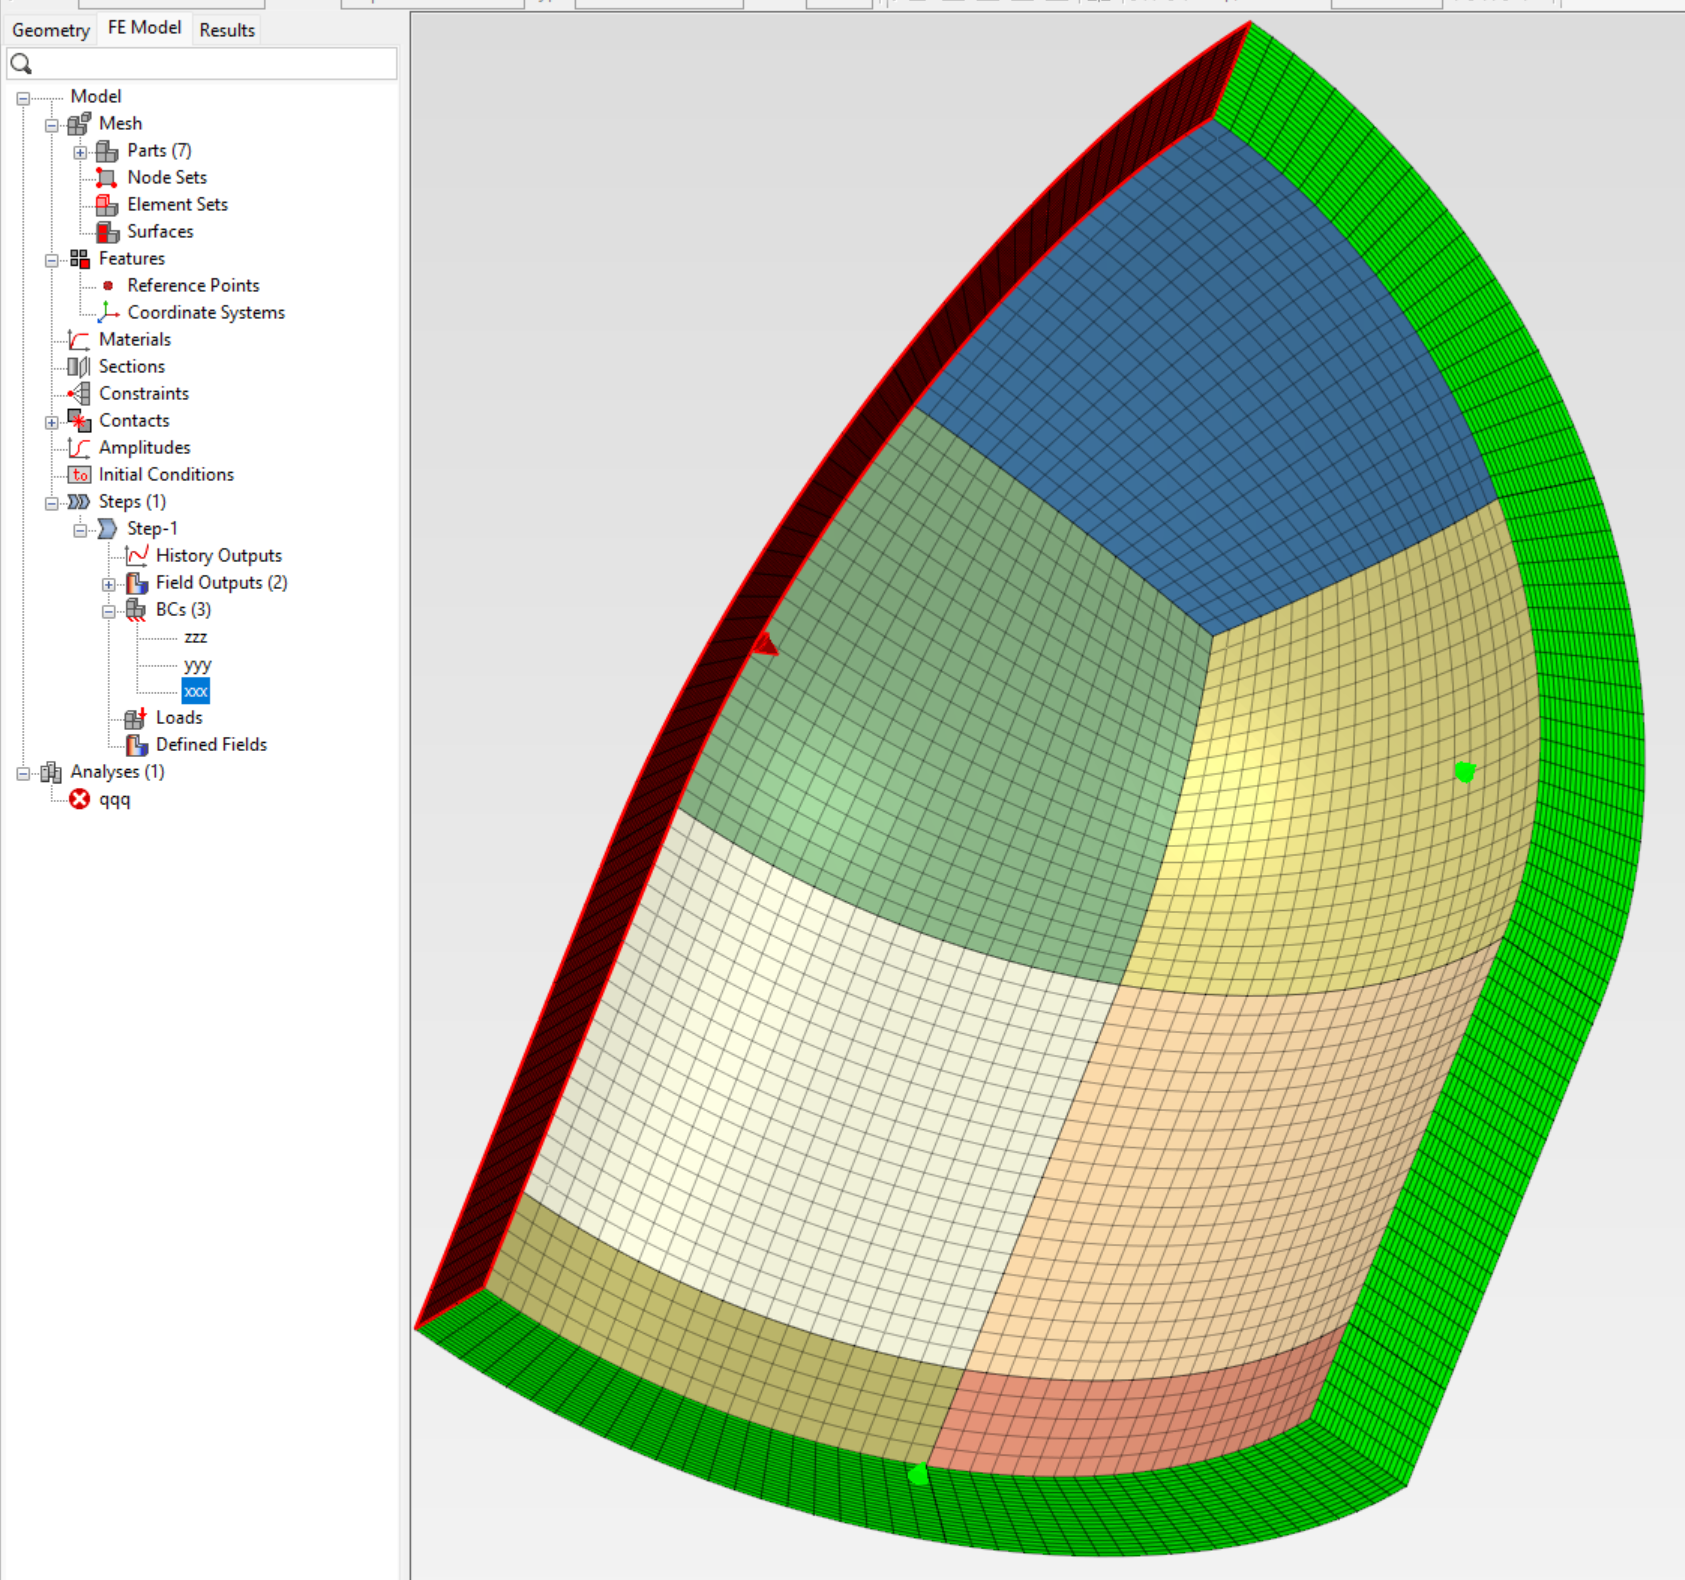
\includegraphics[keepaspectratio,scale=0.30]{images/sc12.png}}
            \only<2>{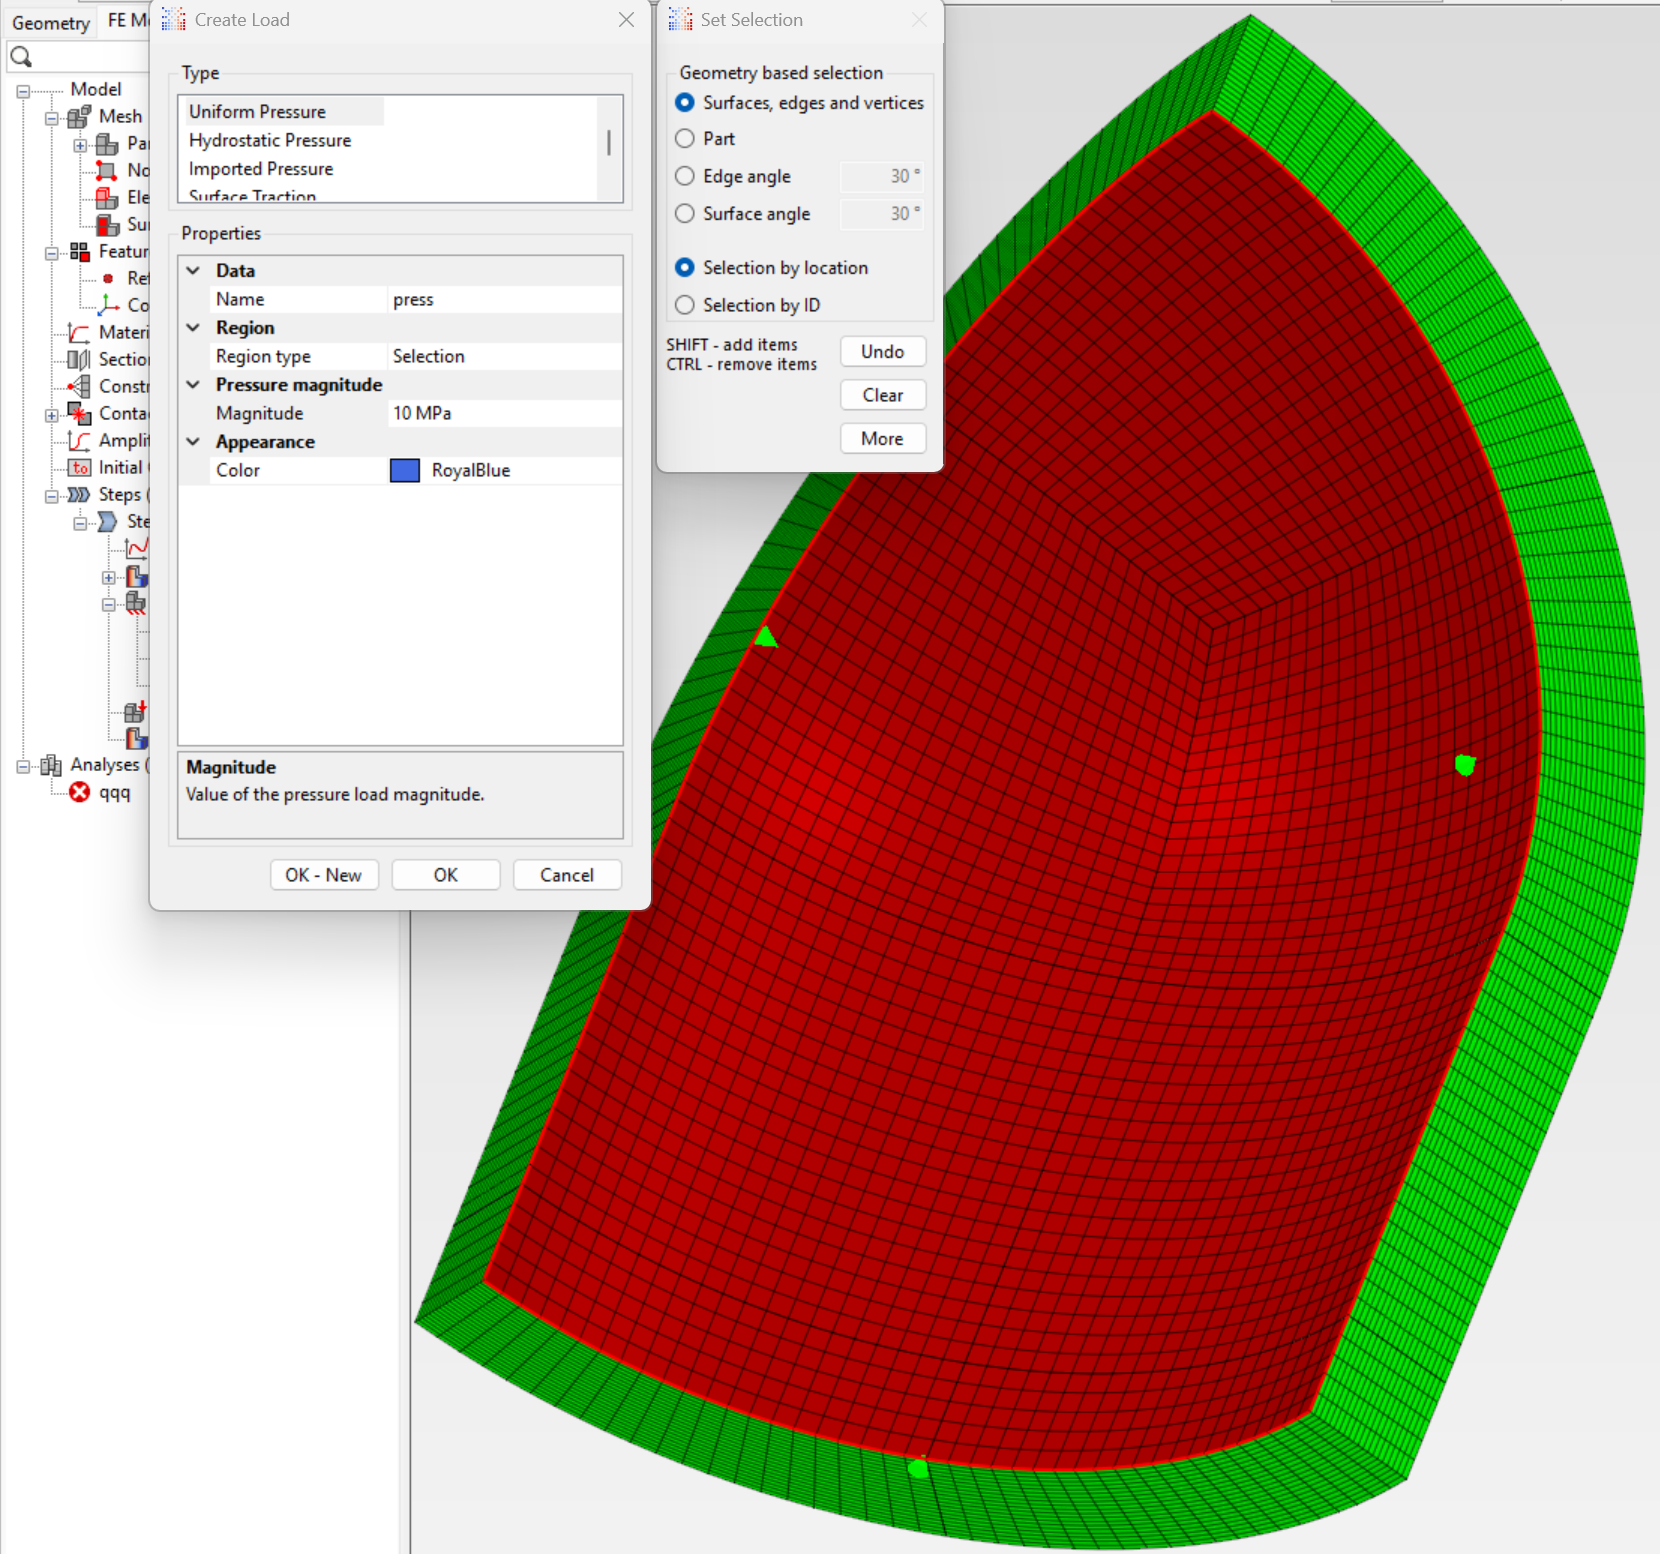
\includegraphics[keepaspectratio,scale=0.30]{images/sc13.png}}
            \caption{境界条件の概要}
          \end{overlayarea}
        \end{center}
      \end{figure}
    \end{column}
  \end{columns}
  \only<1>{
    \begin{textblock*}{160pt}(180pt,103pt)
      \begin{tikzpicture}
         \node[rectangle,fill=cud_yellow,text width=90pt,text centered,rounded corners,minimum height=20pt](s) at (1cm,3.0cm) { \scriptsize x方向固定};
         \draw[->, draw=cud_red, line width=1pt] (75pt,95pt) -- (125pt,130pt);
         \node[rectangle,fill=cud_yellow,text width=90pt,text centered,rounded corners,minimum height=20pt](s) at (2cm,1.2cm) { \scriptsize y方向固定};
         \draw[->, draw=cud_red, line width=1pt] (105pt,35pt) -- (125pt,40pt);
         \node[rectangle,fill=cud_yellow,text width=90pt,text centered,rounded corners,minimum height=20pt](s) at (7cm,0.0cm) { \scriptsize z方向固定};
         \draw[->, draw=cud_red, line width=1pt] (230pt,10pt) -- (225pt,90pt);
      \end{tikzpicture}
    \end{textblock*}
  }
	  \only<2>{
    \begin{textblock*}{160pt}(195pt,75pt)
      \begin{tikzpicture}
         \node[rectangle,fill=cud_yellow,text width=90pt,text centered,rounded corners,minimum height=40pt](s) at (1cm,0cm) { \scriptsize 面圧10MPa};
         \draw[->, draw=cud_red, line width=1pt] (10pt,20pt) -- (78pt,100pt);
         \draw[->, draw=cud_red, line width=1pt] (76pt,20pt) -- (130pt,30pt);
      \end{tikzpicture}
    \end{textblock*}
  }
\end{frame}
